\documentclass[onecolumn, draftclsnofoot,10pt, compsoc]{IEEEtran}
\usepackage[utf8]{inputenc}
\usepackage{graphicx}
\graphicspath{ {./} }
\usepackage{caption}
\usepackage{url}
\usepackage{setspace}
%\usepackage{parskip}
\usepackage{longtable}
\usepackage{hyperref}
\hypersetup{
    colorlinks=true,
    linkcolor=blue,
    filecolor=magenta,      
    urlcolor=blue,
}

\usepackage{geometry}
\geometry{textheight=9.5in, textwidth=7in}

% 1. Fill in these details
\title{User Guide}
\author{Group 73: Stephen Hoffmann, Stewart Rodger, Nicholas Pugliese, Kyle Tyler, Symon Ramos}
\date{February 2019}
\def \CapstoneTeamName{		    Group 73: VR Press}
\def \CapstoneTeamNumber{		73}
\def \GroupMemberOne{			Symon Ramos}
\def \GroupMemberTwo{			Stephen Hoffman}
\def \GroupMemberThree{			Nicholas Pugliese}
\def \GroupMemberFour{			Stewart Rodger}
\def \GroupMemberFive{			Kyle Tyler}
\def \CapstoneProjectName{		Developing Virtual Reality Based Training Experiences for HP's PageWide Web Press Product Line}
\def \CapstoneSponsorCompany{	HP Inc}
\def \CapstoneSponsorPerson{		Tim Holt}



% 2. Uncomment the appropriate line below so that the document type works
\def \DocType{		
				User Guide
				}
			
\newcommand{\NameSigPair}[1]{\par
\makebox[2.75in][r]{#1} \hfil 	\makebox[3.25in]{\makebox[2.25in]{\hrulefill} \hfill		\makebox[.75in]{\hrulefill}}
\par\vspace{-12pt} \textit{\tiny\noindent
\makebox[2.75in]{} \hfil		\makebox[3.25in]{\makebox[2.25in][r]{Signature} \hfill	\makebox[.75in][r]{Date}}}}
% 3. If the document is not to be signed, uncomment the RENEWcommand below
%\renewcommand{\NameSigPair}[1]{#1}

%%%%%%%%%%%%%%%%%%%%%%%%%%%%%%%%%%%%%%%
\begin{document}
\maketitle
\begin{figure}[ht!]
    \centering
    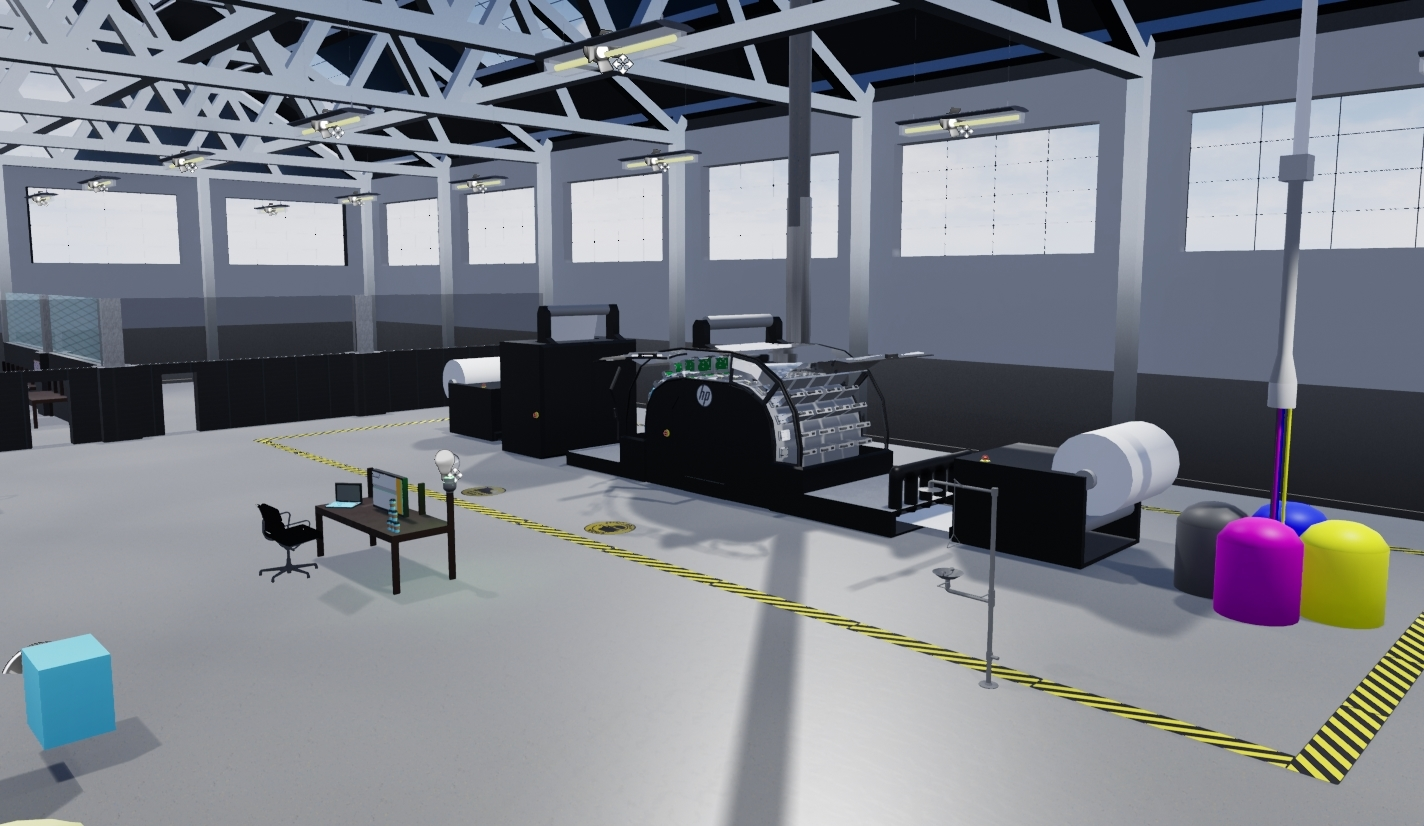
\includegraphics[width=0.85\textwidth]{environment.png}
    \caption{The Virtual Reality Environment}
    \label{fig:printerModel}
\end{figure}

    \begin{abstract}
    % Copied from group problem statement
   This document is a guide for the Virtual Reality (VR) training simulation created by Capstone Group 73: Virtual Reality Printing and designed to train personnel on how to operate aspects of the machinery from HP's PageWide Web Press production line and serve as a feasibility prototype to replace all or part of their current training program. Included are installation instructions, a description of compatible hardware, a general overview of the project, basic controls, and an overview of the user interface. 
   
    \end{abstract}
\newpage
\pagenumbering{arabic}
\tableofcontents
% 7. uncomment this (if applicable). Consider adding a page break.
%\listoffigures
%\listoftables
\clearpage


% Actual Outline of User Guide: 

\section{Required Software and Hardware}

The following hardware items are required to successfully run the application:

\begin{itemize}
    \item A Laptop with the following:
        \begin{itemize}
            \item Windows 10 Operating System or later
            \item Intel® Core™ i5 or better
            \item AMD Ryzen 5 1400 3.4Ghz quad core or better
            \item At least 8GB of RAM
            \item At least 10 GB of Disk Space.
            \item Bluetooth 4.0 Support 
        \end{itemize}
    \item Any of the following graphics cards: 
        \begin{itemize}
            \item Integrated Intel HD Graphics 620 or greater 
            \item DX12-capable integrated GPU
            \item Nvidia MX150 discrete GPU
            \item Nvidia GeForce GTX 1050 discrete GPU
            \item Nvidia 965M discrete GPU
            \item AMD Radeon RX 460/560
        \end{itemize}
    \item A Windows Mixed Reality Headset
    \item A Pair of Windows Mixed Reality Controllers
    \item A Bluetooth Dongle
\end{itemize}


In addition, the following software applications are also required: 
\begin{itemize}
    \item Steam 
        \begin{itemize}
            \item Steam VR Windows Headset Extension
        \end{itemize}
    \item Unreal Engine %FIXME: Put Unreal Version
    \item Windows Mixed Reality Drivers (which will be installed upon first-time use of the headset)
\end{itemize}

\section{Installation Guide}
\subsection{Download the Project}

Our project can be found on GitHub with the following link:

\noindent
\href{https://github.com/SilverGekko/cs461}{https://github.com/SilverGekko/cs461}\\

\noindent
The Executable file can be found under the "releases" section of the github page.

%\noindent In order to download the project to your local computer, please use the GitHub interface or run the following command on your terminal: 
\\
%git clone https://github.com/SilverGekko/cs461.git

In order to test the application, download the zip file from the releases page: Releases->CodeFreeze, unzip it, and run the executable file called "PressVR" contained within the subfoler "WindowsNoEditor."

\subsection{Configure the Windows Mixed Reality Headset}

Please refer to the link to the official setup guide below in order to successfully configure the Windows Mixed Reality Headset.

\noindent
\href{https://support.microsoft.com/en-us/help/4043101/windows-10-set-up-windows-mixed-reality}{https://support.microsoft.com/en-us/help/4043101/windows-10-set-up-windows-mixed-reality}\\

Here are additional resources to assist in the installation of the Windows Mixed Reality environment onto your computer. 

\noindent
\href{https://www.windowscentral.com/how-set-your-windows-mixed-reality-headset}{https://www.windowscentral.com/how-set-your-windows-mixed-reality-headset}\\
\noindent
\href{https://help.irisvr.com/hc/en-us/articles/115015806747-First-Time-Setup-with-Windows-Mixed-Reality-MR-Headsets}{https://help.irisvr.com/hc/en-us/articles/115015806747-First-Time-Setup-with-Windows-Mixed-Reality-MR-Headsets}\\

\subsection{Ensure Steam VR is used}

First, make sure Steam is installed on the current system:

\noindent
\href{https://store.steampowered.com/about/}{https://store.steampowered.com/about/}

\noindent
The Steam VR Plugin can be found here: 

\noindent 
\href{https://store.steampowered.com/app/719950/Windows_Mixed_Reality_for_SteamVR/}{https://store.steampowered.com/app/719950/Windows\_Mixed\_Reality\_for\_SteamVR/}\\

\begin{figure}[ht!]
    \centering
    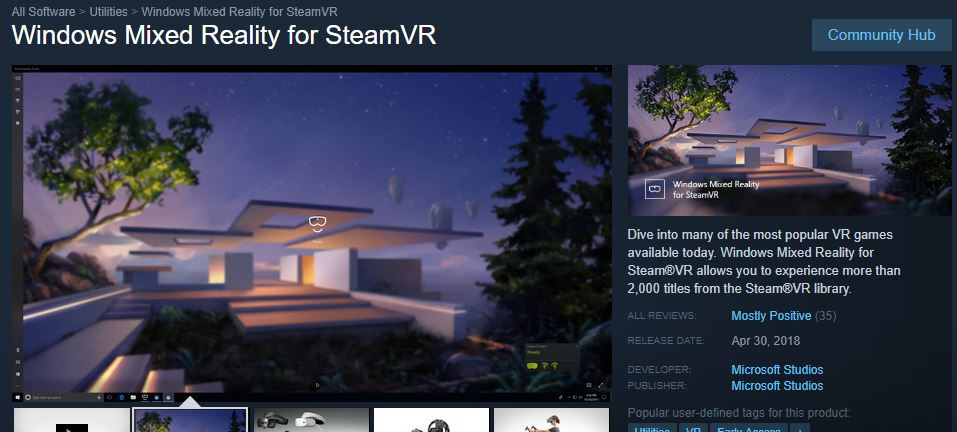
\includegraphics[width=0.85\textwidth]{steamplugin.JPG}
    \caption{Steam VR Plugin}
    \label{fig:printerModel}
\end{figure}

\subsection{Launch Project}

After performing the steps above, please perform the following in order to successfully launch the project: 
\begin{itemize}
    \item Find the executable file within the release zip file: PressVR->WindowsNoEditor->PressVR.exe
\end{itemize}

Once the game has launched put on the headset, pick up the controllers, and refer to section 6 for a description of the scenario.


\section{Basic Controls}
 Figure \ref{fig:controllers} is a description of the project's controller scheme.

\begin{figure}[ht!]
    \centering
    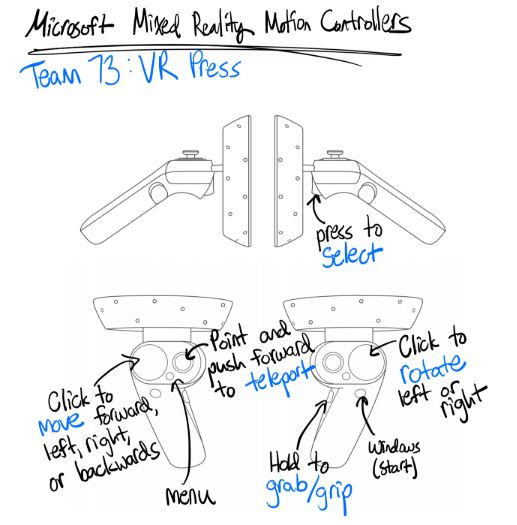
\includegraphics[width=0.85\textwidth]{VRPressInfographic.JPG}
    \caption{Windows Mixed Reality Controller Scheme}
    \label{fig:controllers}
\end{figure}


\subsection{Environment}

\begin{figure}[ht!]
    \centering
    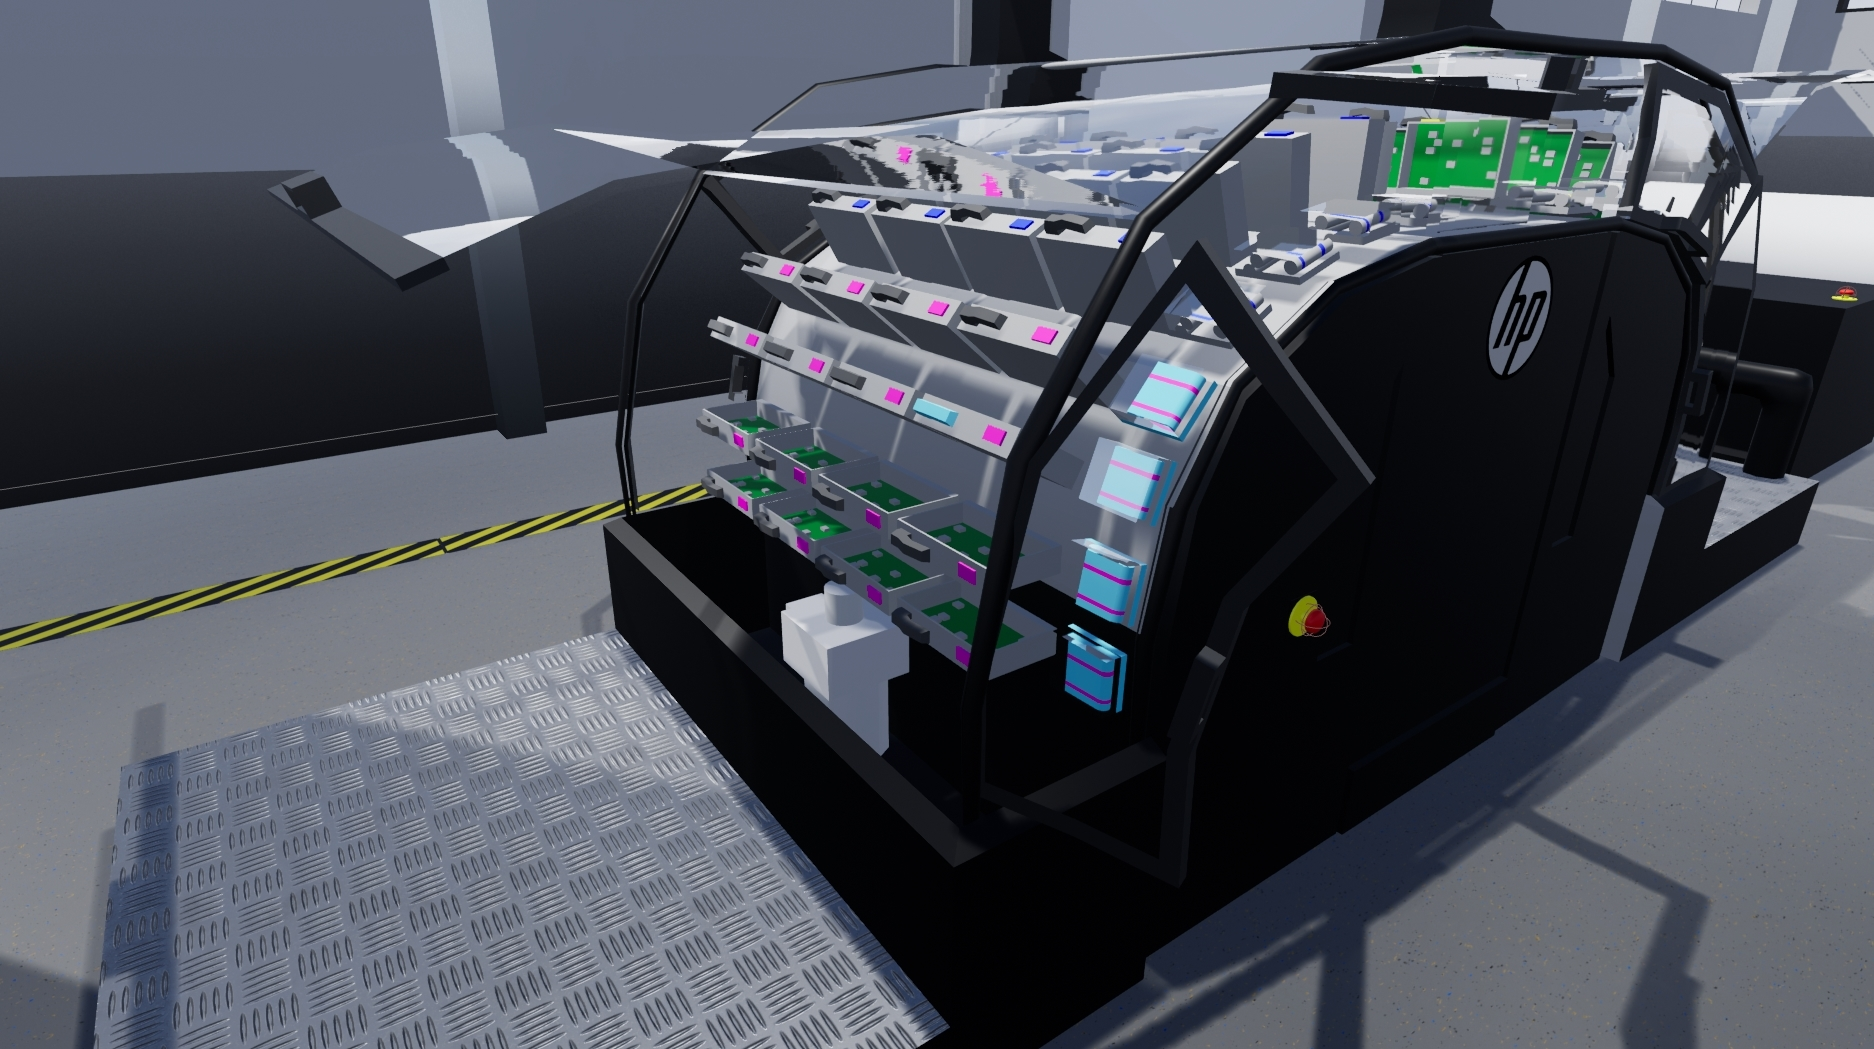
\includegraphics[width=0.85\textwidth]{press1.png}
    \caption{Web Press Printer 3D Model}
    \label{fig:printerModel}
\end{figure}

The entire virtual environment is a 3D model of a warehouse. Models we have added include the Web Press printer itself (modeled after the T240 model), ink barrels, computers, desks, chairs, an office space to serve as our tutorial room, lights, E-Stop buttons, spare printheads, tables, cabinets, and cautionary tape. The Web Press printer is comprised of multiple models, including the printer itself, the winder and unwinder (which is where the paper is fed in and out respectively), and individual printheads of different colors. 

We have also implemented basic functionality with the buttons on the Web Press and the ability to toggle lights on the printer. This is indicated in the figure below: 

\begin{figure}[ht!]
    \centering
    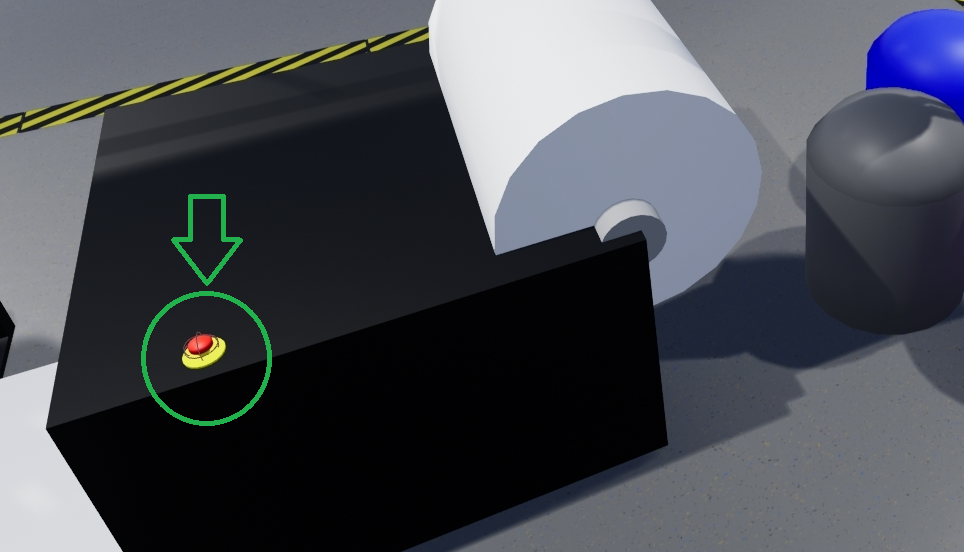
\includegraphics[width=0.85\textwidth]{button.png}
    \caption{The Emergency Stop Button}
    \label{fig:stopbutton}
\end{figure}

\section{Tutorial Scenario}

We have implemented a tutorial mode (created in the office space of our environment) in which the user will be tasked with performing basic actions in a cohesive narrative. 

\begin{figure}[ht!]
    \centering
    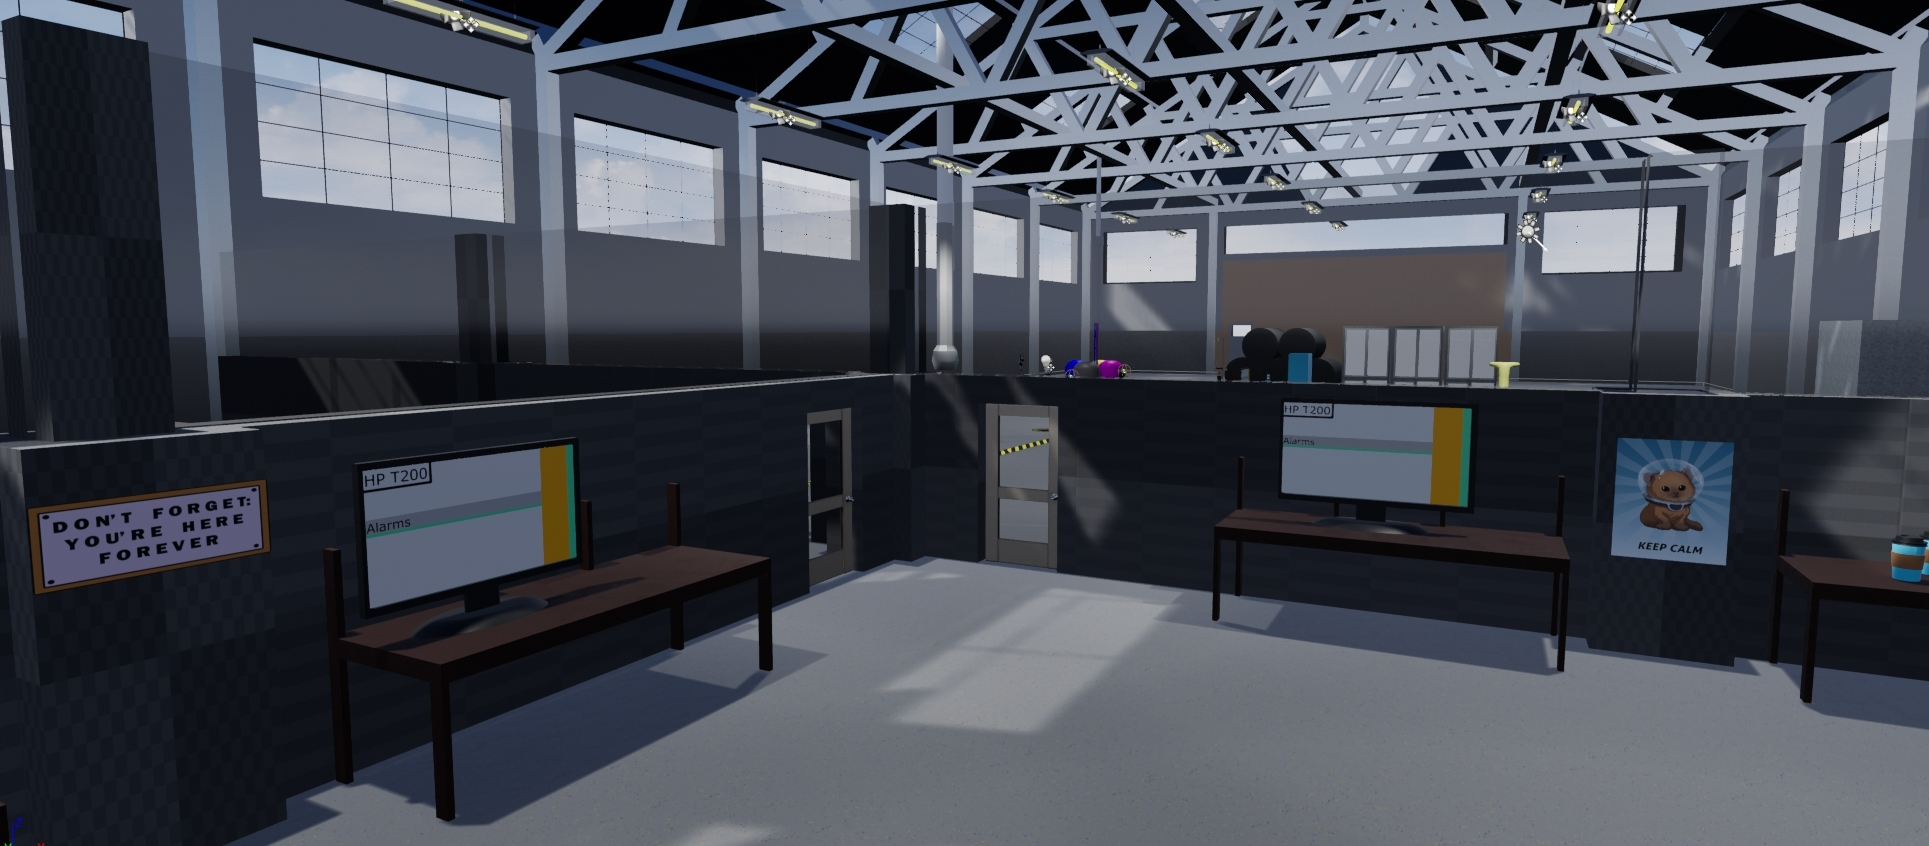
\includegraphics[width=0.85\textwidth]{tutorialSpace.png}
    \caption{The Tutorial Environment}
    \label{fig:tutorial}
\end{figure}


In this tutorial space, the user are asked to look around, focus their screen towards something, move around, grab items, and interact with the environment. 
All users are given the option of going through the tutorial mode before attempting the training module.

There are three main tutorial sections to illustrate the basic skills needed to use the Virtual Reality program:

\begin{itemize}
    \item Looking around the room in VR ("Seeing" tutorial)
    \item Using the hand-held controllers to teleport ("Moving" tutorial)
    \item Picking up objects and pressing buttons ("Interacting" tutorial)
\end{itemize}

Each of these tutorials takes places in a section of the environment designed to look like an office cubicle. This tutorial space takes place in a separate level than the Web Press itself. The user may leave this tutorial level and go to the main Web Press level by clicking a button on the user interface. The tutorial instructs the user to do this once the three tutorials listed above are done, but an experienced user may exit the tutorial at any time by accessing the same menu.

\subsubsection{Sight}
The seeing tutorial teaches the user that they may look around with full 3D motion while wearing the headset. The tutorial is completed by making the user point to an onscreen crosshair at a computer monitor on a desk. This process is repeated on three total monitors ranging from in front of the user, to almost directly behind them. The idea is to force the user to physically turn their body around so they learn the extent of the control they have over the viewport with the headset.

\subsubsection{Movement}
The moving tutorial teaches the user that they can move around the virtual space by pressing a button on the controller, pointing, and releasing to teleport to that location. The tutorial is completed when the user teleports away from the starting position. This teaches the user how to move around the environment, which they will need to do to complete the training scenarios.   

\subsubsection{Interaction}
The interacting tutorial teaches the user that there are objects in the virtual environment that may be interacted with using the handheld controllers by moving the controller over the object in the virtual space and holding down the trigger button. All of the objects in the virtual space that may be grabbed like this are colored the same sky blue color as shown in figure \ref{fig:skyblue}.

\begin{figure}[ht!]
    \centering
    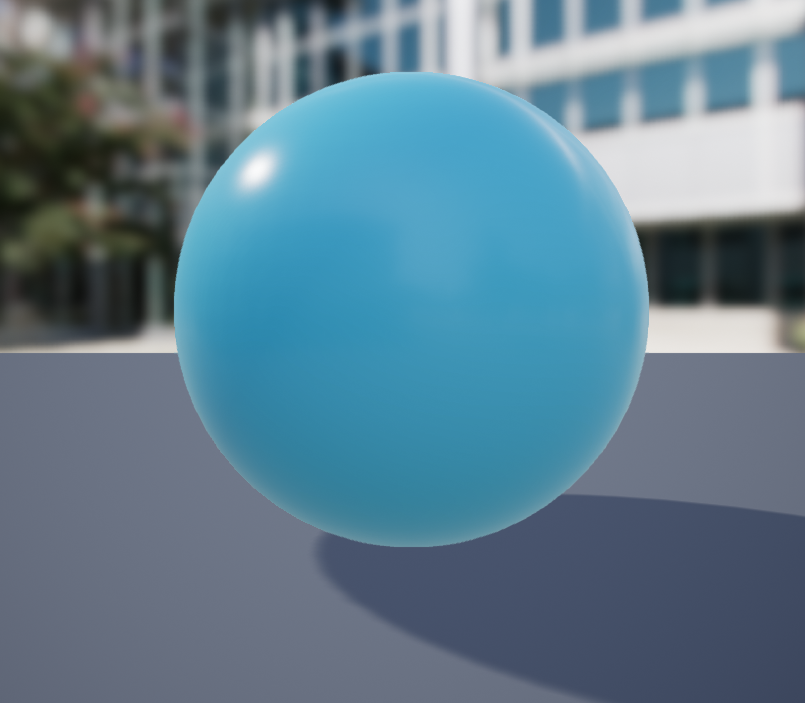
\includegraphics[scale=0.5]{touchMeBlue.png}
    \caption{The specific shade of blue that informs the user they may pick up and manipulate the object.}
    \label{fig:skyblue}
\end{figure}

\section{Training Scenario}

\subsection{Replacing Printheads}

The T2XX Web Press Operating Manual outlines a sequential series of steps that the user has to complete in order to successfully remove the existing printhead and insert the new one. In a later section detailing common troubleshooting scenarios, several scenarios where the replacement of printheads would be applicable are included, such as when a printhead is overheating. Figure 8 below outlines the user workflow of the replacement of printheads. It should be followed until the voice over informs the user that the scenario is complete. If at any point the user gets stuck they may open the menu (see figure 3) and select the training scenario again to restart the scenario.

\begin{figure}[ht!]
    \centering
    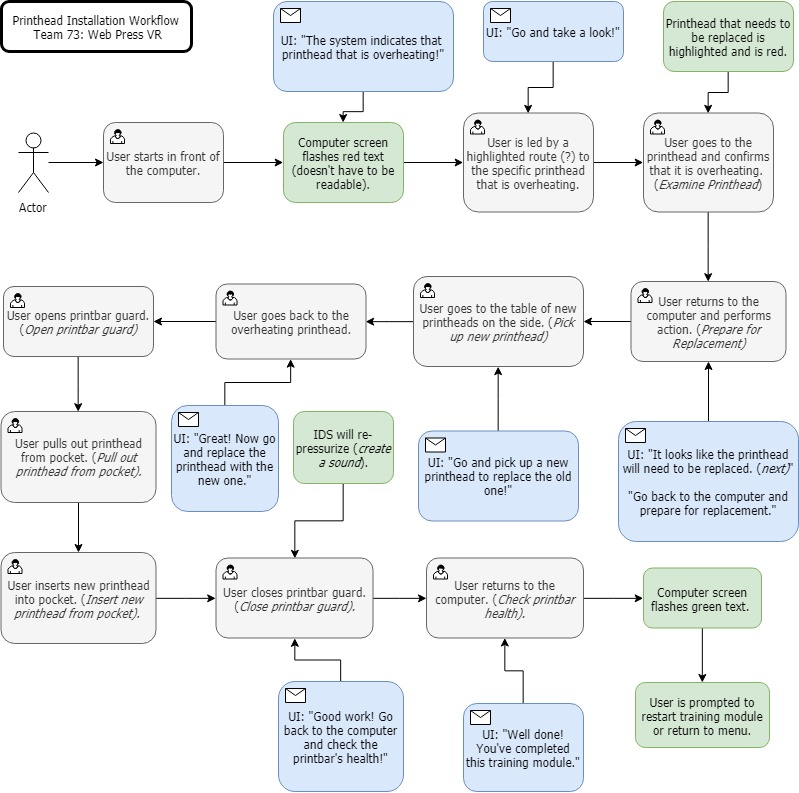
\includegraphics[width=0.85\textwidth]{PrintheadInstallationWorkflow.jpg}
    \caption{The Printhead Installation Workflow}
    \label{fig:workflow}
\end{figure}
\section{Developer Notes}

Please contact HP personnel for more information and inquiries should further development be desired.

Future Implementation that could be considered is as follows: 
\begin{itemize}
    \item Additional training scenarios, such as the replacement of printer wiper cassettes.
    \item Refinement of 3D environment.
    \item Support for additional headsets.
    \item Additional Web Press Models. 
    \item An expanded warehouse environment that includes office space.
\end{itemize}

\section{Version Log}
This document was last updated on 4/14/19.


\end{document}